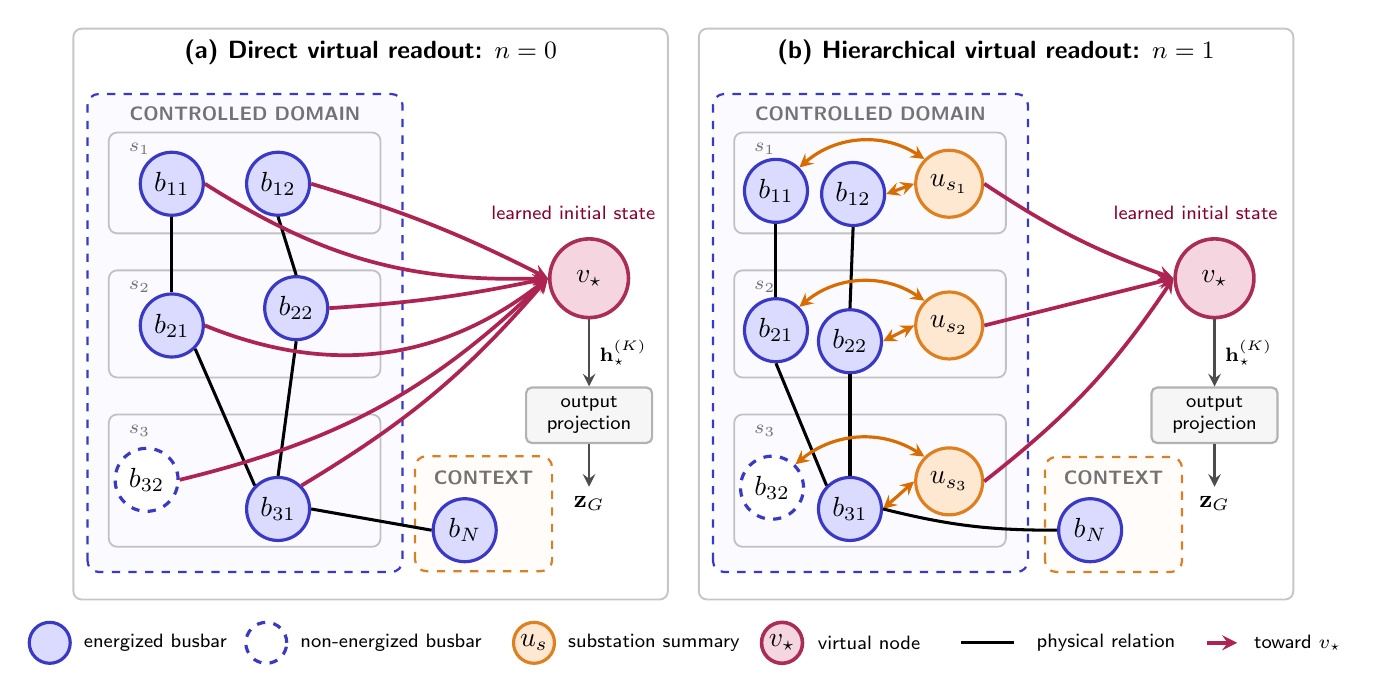
\begin{tikzpicture}[
  x=1cm,
  y=1cm,
  >=stealth,
  font=\sffamily,
  busbar/.style={
    circle,
    draw=blue!55!gray,
    fill=blue!14,
    line width=1.15pt,
    minimum size=8mm,
    inner sep=0pt
  },
  busbaroff/.style={
    circle,
    draw=blue!55!gray,
    fill=white,
    dashed,
    line width=1.15pt,
    minimum size=8mm,
    inner sep=0pt
  },
  summary/.style={
    circle,
    draw=orange!75!gray,
    fill=orange!18,
    line width=1.15pt,
    minimum size=8.5mm,
    inner sep=0pt
  },
  virtual/.style={
    circle,
    draw=purple!65!gray,
    fill=purple!16,
    line width=1.3pt,
    minimum size=10mm,
    inner sep=0pt
  },
  output/.style={
    draw=gray!60,
    fill=gray!7,
    rounded corners=2pt,
    line width=0.8pt,
    minimum width=16mm,
    minimum height=7mm,
    font=\scriptsize\sffamily,
    align=center
  },
  physical/.style={draw=black, line width=1.1pt},
  summaryedge/.style={<->, draw=orange!85!black, line width=1.15pt},
  virtualedge/.style={->, draw=purple!72!gray, line width=1.35pt},
  readoutedge/.style={->, draw=black!70, line width=1pt},
  panel/.style={draw=gray!45, rounded corners=3pt, line width=0.7pt},
  controlled/.style={
    draw=blue!55!gray,
    dashed,
    rounded corners=4pt,
    fill=blue!2,
    line width=0.8pt
  },
  context/.style={
    draw=orange!70!gray,
    dashed,
    rounded corners=4pt,
    fill=orange!2,
    line width=0.8pt
  },
  subbox/.style={draw=gray!48, rounded corners=3pt, line width=0.65pt},
  zone/.style={font=\scriptsize\bfseries\sffamily, text=gray!75},
  title/.style={font=\small\bfseries\sffamily},
  note/.style={font=\scriptsize\sffamily, align=center},
  muted/.style={font=\scriptsize\itshape\sffamily, align=center, text=gray!62}
]

% ---------------------------------------------------------------------------
% (a) Direct busbar-to-virtual readout
% ---------------------------------------------------------------------------
\path[context] (12.34,0.35) rectangle (14.08,1.81);
\begin{scope}[xshift=0cm]
  \path[panel] (0,0) rectangle (7.55,7.25);
  \node[title] at (3.775,6.95) {(a) Direct virtual readout: $n=0$};
  \path[controlled] (0.18,0.35) rectangle (4.18,6.42);
  \node[zone, text=black!55] at (2.18,6.17) {CONTROLLED DOMAIN};
  \path[context] (4.34,0.36) rectangle (6.08,1.82);
  \node[zone, text=black!55] at (5.21,1.55) {CONTEXT};

  \path[subbox] (0.45,4.65) rectangle (3.90,5.93);
  \path[subbox] (0.45,2.82) rectangle (3.90,4.18);
  \path[subbox] (0.45,0.67) rectangle (3.90,2.35);
  \node[note, anchor=west, text=black!55] at (0.58,5.72) {$s_1$};
  \node[note, anchor=west, text=black!55] at (0.58,3.97) {$s_2$};
  \node[note, anchor=west, text=black!55] at (0.58,2.14) {$s_3$};

  \node[busbar] (d-b11) at (1.25,5.28) {$b_{11}$};
  \node[busbar] (d-b12) at (2.60,5.28) {$b_{12}$};
  \node[busbar] (d-b21) at (1.25,3.48) {$b_{21}$};
  \node[busbar] (d-b22) at (2.83,3.7) {$b_{22}$};
  \node[busbar] (d-b31) at (2.60,1.15) {$b_{31}$};
  \node[busbaroff] (d-b32) at (0.93,1.52) {$b_{32}$};
  \node[busbar] (d-bn) at (4.97,0.88) {$b_N$};

  \draw[physical] (d-b11.south) -- (d-b21.north);
  \draw[physical] (d-b12.south) -- (d-b22.north);
  \draw[physical] (d-b21.south east) -- (d-b31.north west);
  \draw[physical] (d-b22.south) -- (d-b31.north);
  \draw[physical] (d-b31.east) -- (d-bn.west);

  \node[virtual] (d-v) at (6.55,4.08) {$v_\star$};
  \node[note, text=purple!70!black] at (6.35,4.91) {learned initial state};
  \draw[virtualedge] (d-b11.east) to[bend right=17] (d-v.west);
  \draw[virtualedge] (d-b12.east) to[bend left=5] (d-v.west);
  \draw[virtualedge] (d-b21.east) to[bend right=30] (d-v.west);
  \draw[virtualedge] (d-b22.east) to[bend right=4] (d-v.west);
  \draw[virtualedge] (d-b31.north east) to[bend right=9] (d-v.west);
  \draw[virtualedge] (d-b32.east) to[bend right=15] (d-v.west);

  \node[output] (d-out) at (6.55,2.34) {output\\projection};
  \node[font=\small] (d-z) at (6.55,1.22) {$\mathbf z_G$};
  \draw[readoutedge] (d-v.south) --
    node[note, right] {$\mathbf h_\star^{(K)}$} (d-out.north);
  \draw[readoutedge] (d-out.south) -- (d-z.north);
\end{scope}
\begin{scope}[xshift=226pt]
  \path[panel] (0,0) rectangle (7.55,7.25);
  \node[title] at (3.775,6.95) {(b) Hierarchical virtual readout: $n=1$};
  \path[controlled] (0.18,0.35) rectangle (4.18,6.42);
  \node[zone, text=black!55] at (2.18,6.17) {CONTROLLED DOMAIN};
  \path[subbox] (0.45,4.65) rectangle (3.90,5.93);
  \path[subbox] (0.45,2.82) rectangle (3.90,4.18);
  \path[subbox] (0.45,0.67) rectangle (3.90,2.35);
  \node[note, anchor=west, text=black!55] at (0.58,5.72) {$s_1$};
  \node[note, anchor=west, text=black!55] at (0.58,3.97) {$s_2$};
  \node[note, anchor=west, text=black!55] at (0.58,2.14) {$s_3$};
  \node[busbar] (h-b11) at (0.98,5.19) {$b_{11}$};
  \node[busbar] (h-b12) at (1.96,5.15) {$b_{12}$};
  \node[summary] (h-u1) at (3.18,5.28) {$u_{s_1}$};
  \node[busbar] (h-b21) at (0.98,3.42) {$b_{21}$};
  \node[busbar] (h-b22) at (1.92,3.28) {$b_{22}$};
  \node[summary] (h-u2) at (3.18,3.48) {$u_{s_2}$};
  \node[busbar] (h-b31) at (1.92,1.15) {$b_{31}$};
  \node[busbaroff] (h-b32) at (0.93,1.42) {$b_{32}$};
  \node[summary] (h-u3) at (3.18,1.50) {$u_{s_3}$};
  \draw[physical] (h-b11.south) -- (h-b21.north);
  \draw[physical] (h-b12.south) -- (h-b22.north);
  \draw[physical] (h-b21.south) -- (h-b31.north west);
  \draw[physical] (h-b22.south) -- (h-b31.north);
  \draw[summaryedge] (h-b11.north east) to[bend left=37] (h-u1.north west);
  \draw[summaryedge] (h-b12.east) -- (h-u1.west);
  \draw[summaryedge] (h-b21.north east) to[bend left=37] (h-u2.north west);
  \draw[summaryedge] (h-b22.east) -- (h-u2.west);
  \draw[summaryedge] (h-b31.east) -- (h-u3.west);
  \draw[summaryedge] (h-b32.north east) to[bend left=36] (h-u3.north west);
  \node[virtual] (h-v) at (6.55,4.08) {$v_\star$};
  \node[note, text=purple!70!black] at (6.31,4.91) {learned initial state};
  \draw[virtualedge] (h-u1.east) to[bend left=-7] (h-v.west);
  \draw[virtualedge] (h-u2.east) -- (h-v.west);
  \draw[virtualedge] (h-u3.east) to[bend right=9] (h-v.west);
  \node[output] (h-out) at (6.55,2.34) {output\\projection};
  \node[font=\small] (h-z) at (6.55,1.22) {$\mathbf z_G$};
  \draw[readoutedge] (h-v.south) --
    node[note, right] {$\mathbf h_\star^{(K)}$} (h-out.north);
  \draw[readoutedge] (h-out.south) -- (h-z.north);
  \node[busbar] (h-bn) at (4.97,0.88) {$b_N$};
  \draw[physical] (h-b31.east) to[bend left=-7] (h-bn.west);
\end{scope}
\node[busbar, minimum size=5.2mm] at (-0.3,-0.55) {};
\node[note, anchor=west] at (0.01,-0.55) {energized busbar};
\node[busbaroff, minimum size=5.2mm] at (2.45,-0.55) {};
\node[note, anchor=west] at (2.76,-0.55) {non-energized busbar};
\node[summary, minimum size=5.2mm] at (5.85,-0.55) {$u_s$};
\node[note, anchor=west] at (6.16,-0.55) {substation summary};
\node[virtual, minimum size=5.2mm] at (9,-0.55) {$v_\star$};
\node[note, anchor=west] at (9.33,-0.55) {virtual node};
\draw[physical] (11.27,-0.55) -- (11.95,-0.55);
\node[note, anchor=west] at (12.11,-0.55) {physical relation};
\draw[virtualedge] (14.4,-0.55) -- (14.78,-0.55);
\node[note] at (15.55,-0.55) {toward $v_\star$};
\node[zone, text=black!55] at (13.21,1.54) {CONTEXT};
\end{tikzpicture}
